The implementation and testing of the sentiment analysis tool \citep{sentimentanalysistool} have yielded valuable insights into the functionality and performance of the developed software. The purpose of this chapter is to present a software evaluation, encompassing the evaluation of key components of the system, such as sentiment analysis, social media interfacing, data management, and the GUI. Furthermore, it discusses the details of fulfillment for the previously outlined functional and non-functional requirements of the application from the requirements analysis, followed by further reflection on the development process and possible areas for improvement.

\section{Software Evaluation}
    \subsection{Sentiment Analysis Model}
    The sentiment analysis model is the core component of the application, aimed at classifying the sentiment of social media posts into positive, and negative categories. While PFDualBERT was not implemented, BERT saw great success in terms of accuracy and other metrics.

    Initially BERT model was trained on a dataset containing 1,600,000 rows over 3 epochs and with a learning rate of 2e-5. This proved successful according to the predefined requirements of this project, showing accuracy of 86.95\% during testing. However, the model took 48,755 seconds to complete training, along with a further 519 seconds of testing; this is entirely impractical as this inhibits further fine-tuning that may take place. The training also showed over-fitting taking place, as the training accuracy skyrocketed up to nearly 90\% over each epoch while validation accuracy hovered at ~87\%.

    \FloatBarrier
    \begin{figure}[h]
        \centering
        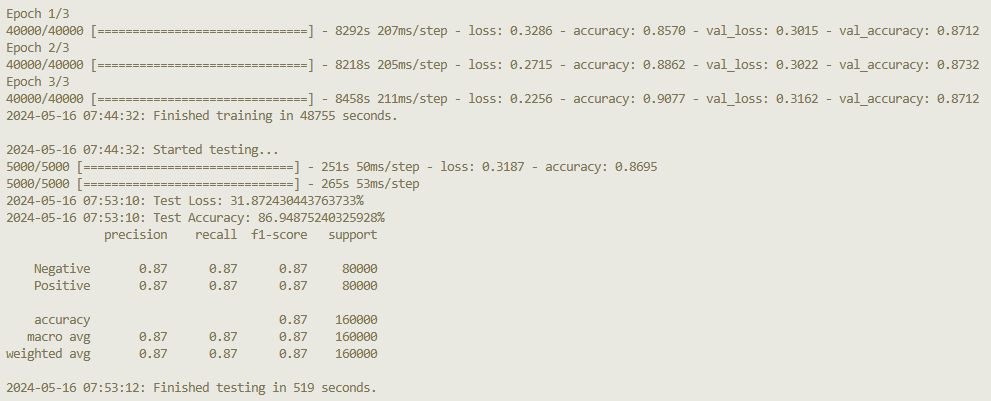
\includegraphics[width=0.95\textwidth]{figures/train-16m-console.png}
        \caption{Standard training results on 1.6 million rows.}
    \end{figure}

    \begin{figure}[h]
        \centering
        \begin{subfigure}{0.49\textwidth}
            \centering
            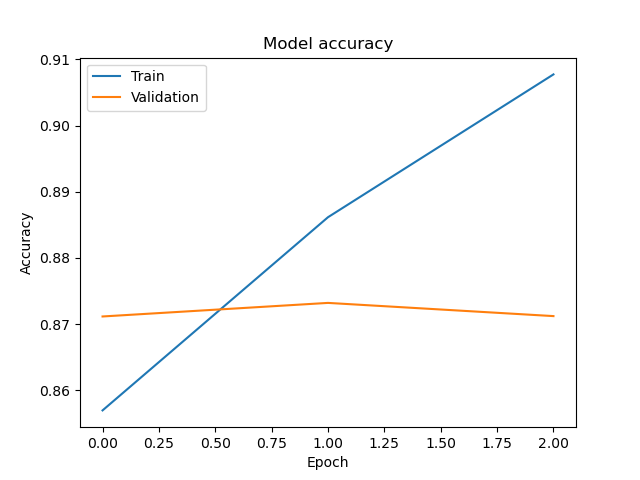
\includegraphics[width=\textwidth]{figures/standard-train-1600000-accuracy.png}
        \end{subfigure}
        \begin{subfigure}{0.49\textwidth}
            \centering
            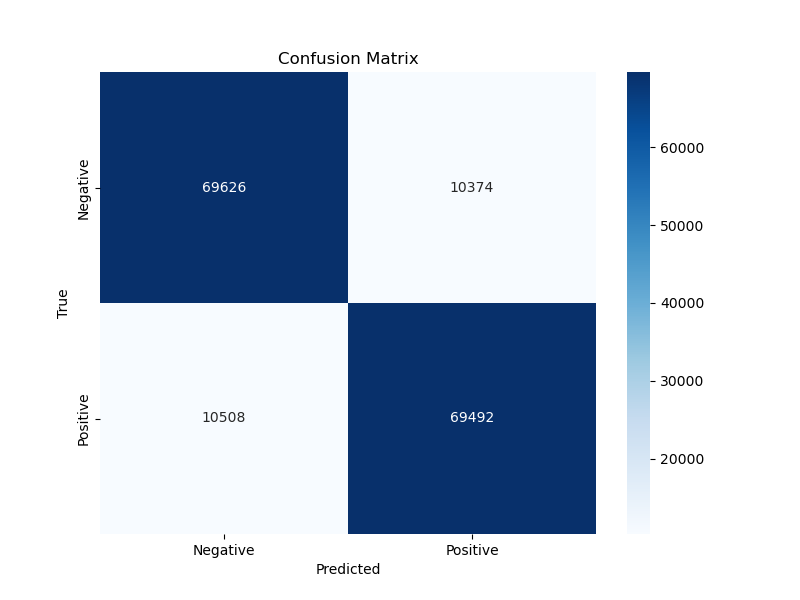
\includegraphics[width=\textwidth]{figures/standard-train-1600000-confusion.png}
        \end{subfigure}
        \caption{Accuracy and confusion matrix for standard training on 1.6 million rows.}
    \end{figure}
    \FloatBarrier

    To combat this, the model was trained using cross-validation with 5 folds and only 5,000 rows of training data. This approach showed great success, proving to have an accuracy of 99.9\% during testing, corresponding train/test accuracy, and only one false positive and one false negative. This conveys that the cross-validation dramatically improved the accuracy and generalisation of the model. It also proved to be significantly faster than training on the full dataset; however, when attempting to train on 10,000 rows, an Out-Of-Memory (OOM) error was thrown, showing that this method uses a large amount of resources when compared to standard training.

    \FloatBarrier
    \begin{figure}[h]
        \centering
        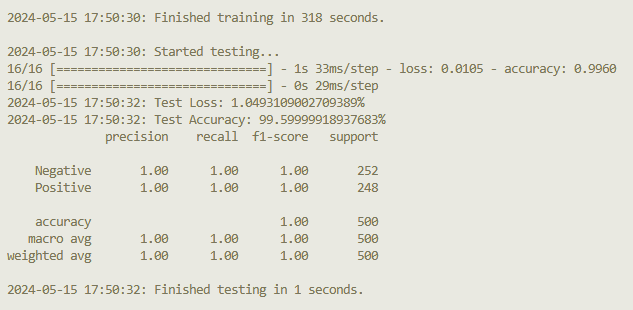
\includegraphics[width=0.95\textwidth]{figures/cross_validation_5000_overall.png}
        \caption{Training results using 5 fold cross-validation on 5,000 rows.}
    \end{figure}

    \begin{figure}[h]
        \centering
        \begin{subfigure}{0.49\textwidth}
            \centering
            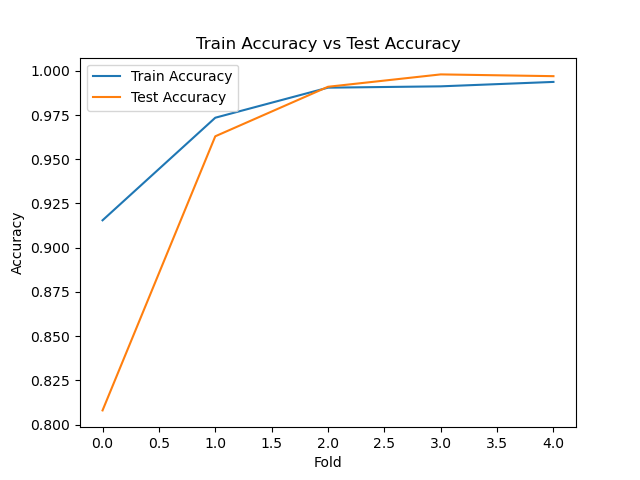
\includegraphics[width=\textwidth]{figures/cross_validation_5000_accuracy.png}
        \end{subfigure}
        \begin{subfigure}{0.49\textwidth}
            \centering
            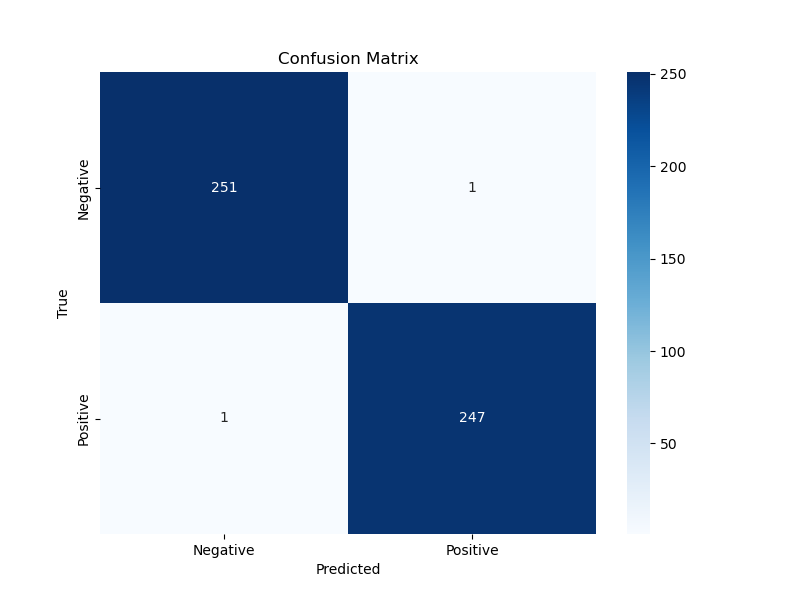
\includegraphics[width=\textwidth]{figures/cross_validation_5000_confusion.png}
        \end{subfigure}
        \caption{Accuracy and confusion matrix for 5 fold cross-validation on 5,000 rows.}
    \end{figure}
    \FloatBarrier

    Finally, an attempt was made at using 3 fold cross-validation with more rows, and it was found that this approach allows training on a dataset of up to 100,000 rows (higher was not attempted). It was found that even with the extra training data, performance actually showed a fractional decrease, with an accuracy of 99.49\%, mainly as there was not much room to improve. This decrease in accuracy should be disregarded due to the many variables at play, however the training execution time should not be ignored; the time taken for this approach was 4,975 seconds, a 93.61\% increase compared to the 318 seconds that the previous approach took, meaning that even though this may increase generalisation, it is inefficient in comparison.

    \FloatBarrier
    \begin{figure}[h]
        \centering
        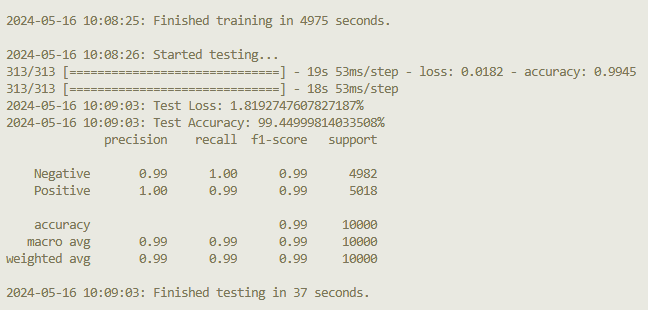
\includegraphics[width=0.95\textwidth]{figures/cross_validation_100000_console_overall_3f.png}
        \caption{Training results using 3 fold cross-validation on 100,000 rows.}
    \end{figure}

    \begin{figure}[h]
        \centering
        \begin{subfigure}{0.49\textwidth}
            \centering
            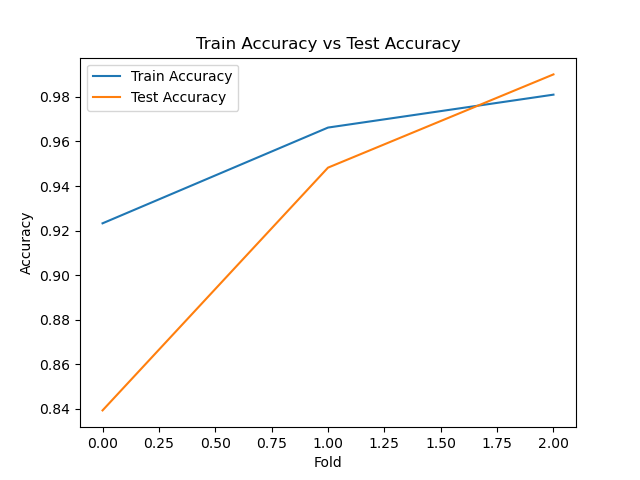
\includegraphics[width=\textwidth]{figures/cross_validation_100000_accuracy_3f.png}
        \end{subfigure}
        \begin{subfigure}{0.49\textwidth}
            \centering
            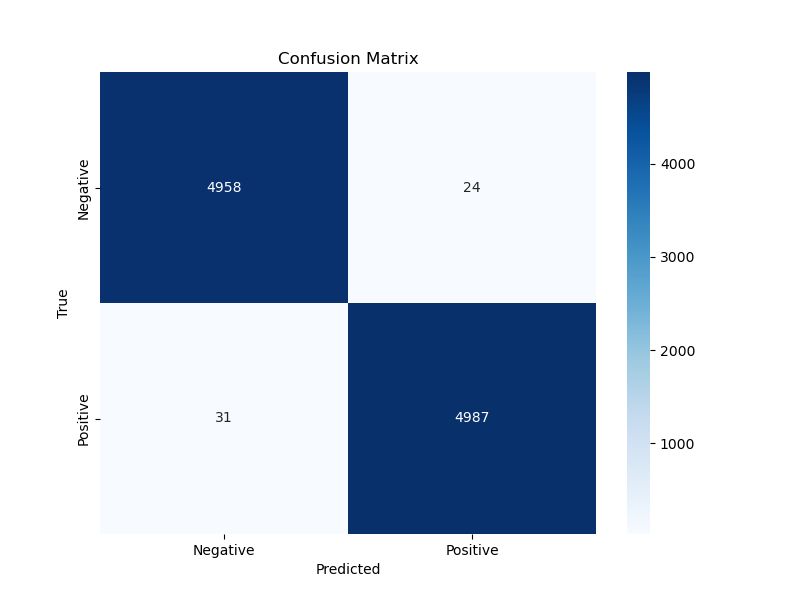
\includegraphics[width=\textwidth]{figures/cross_validation_100000_confusion_3f.png}
        \end{subfigure}
        \caption{Accuracy and confusion matrix for 3 fold cross-validation on 100,000 rows.}
    \end{figure}
    \FloatBarrier

    Finally, the model trained with 5 folds and 5,000 rows of data was tested on entirely unseen data, for this purpose 10 fake Reddit posts were created.

    \begin{python}
reddit_posts = ["Just landed my dream job! [SEP] I can't believe it finally happened. After months of interviews and applications, I got the job I've always wanted. Feeling on top of the world!",
"Had the best meal ever [SEP] Went to this new Italian restaurant downtown and it was amazing. The pasta was to die for and the service was impeccable.",
"Vacation was a blast! [SEP] Just got back from a week-long vacation in Hawaii. The beaches were stunning and the weather was perfect. Highly recommend!",
"Completed my first triathlon [SEP] After months of training, I finished my first triathlon. It was tough but so rewarding. Can't wait to do it again!",
"New hobby is so much fun [SEP] Started learning how to play the guitar and I'm loving it. It's challenging but incredibly satisfying when I nail a new song.",
"Worst customer service ever [SEP] Had a terrible experience at the electronics store. The staff were rude and completely unhelpful. Never going back.",
"Car problems again [SEP] My car broke down for the second time this month. It's so frustrating and costly to keep repairing it. Might have to buy a new one.",
"Disappointing movie night [SEP] Watched a highly anticipated movie and it was a total letdown. The plot was boring and the acting was subpar.",
"Feeling under the weather [SEP] Caught a nasty cold and have been feeling awful all week. Can't wait to get back to my usual self.",
"Bad dining experience [SEP] Went to a new sushi place and got food poisoning. Spent the night feeling miserable. Definitely won't be returning."]
    \end{python}

    When predicting the sentiment of these posts, the model predicted each one correctly, all with >99.9\% confidence, aside from one outlier with 97.13\% confidence.

    \FloatBarrier
    \begin{figure}[h]
        \centering
        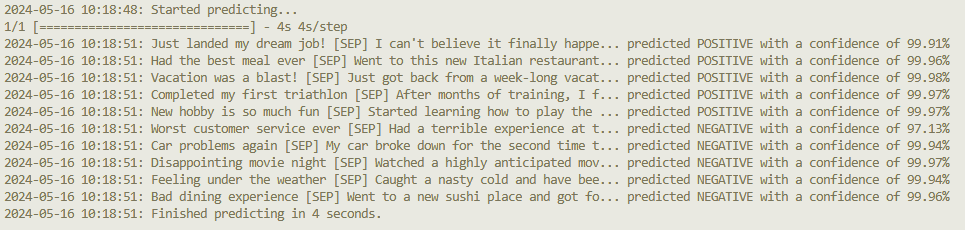
\includegraphics[width=0.95\textwidth]{figures/cross_validation_5000_predictions.png}
        \caption{Unseen predictions on 10 entries with 5 fold cross-validated model.}
    \end{figure}
    \FloatBarrier

    \subsection{Social Media Data Collection}
    To test the social media data collection, the functionality of \pinline{RedditScraper} must be assessed. This was accomplished by performing a simple unit test, to check that the programme is capable of retrieving a post from a specified subreddit with specified search terms, along with its comments.
    \begin{python}
scraper = toolkit.RedditScraper()
posts, comments = scraper.search_sub('machinelearning', ['BERT', 'Transformers'], 1)
print(posts)
for comment in comments:
    print(comment)
    \end{python}

    \FloatBarrier
    \begin{figure}[h]
        \centering
        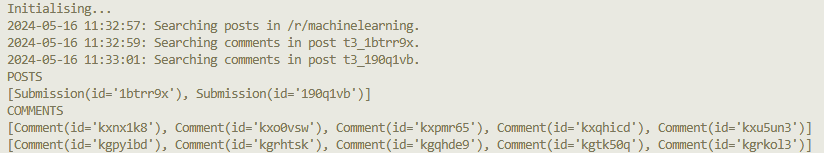
\includegraphics[width=0.95\textwidth]{figures/scrape-test.png}
        \caption{Results of testing social media data collection.}
    \end{figure}
    \FloatBarrier

    The content of these posts was also checked, to be sure that the given search terms were found and in the correct subreddit.

    \begin{python}
for post in posts:
    print(f"SUBREDDIT: {post.subreddit.display_name}")
    print(f"TITLE: {post.title}")
    print(f"BODY: {post.selftext}")
    \end{python}

    \FloatBarrier
    \begin{figure}[ht]
        \begin{minipage}[t]{0.45\textwidth}
            \centering
            \begin{tabular}{|p{7cm}|}
                \hline
                \textbf{/r/machinelearning} \\
                \hline
                \textbf{[D] SOTA BERT-like model?} \\
                \hline
                So we are all probably aware of state-of-the-art decoder only LLMs like GPT-4, Claude etc. These are great for generating text. But what I am not aware of is the SOTA BERT-like model. You know, things that can be used for tasks like NER, POS tagging, token classification. Are there models that are significantly better than say Roberta? \\
                \hline
            \end{tabular}
        \end{minipage}
        \hfill
        \begin{minipage}[t]{0.45\textwidth}
            \centering
            \begin{tabular}{|p{7cm}|}
                \hline
                \textbf{/r/machinelearning} \\
                \hline
                \textbf{[D] So, Mamba vs. Transformers... is the hype real?} \\
                \hline
                Heard all the buzz about Mamba, the new kid on the sequence modeling block. Supposedly it's faster, handles longer sequences better, and even outperforms Transformers on some tasks. But is it really a throne-stealer or just another flash in the pan? \\
                My perception: \\
                Strengths: Mamba boasts efficient memory usage, linear scaling with sequence length, and impressive performance in language and DNA modeling. Plus, it ditches the attention mechanism, potentially paving the way for faster inference. \\
                Weaknesses: Still early days, so Mamba's long-term stability and performance across diverse tasks remain to be seen. And while it doesn't need attention, its state space approach might be trickier to grasp for some folks. \\
                To the AI aficionados out there, is Mamba just the next shiny toy, or a genuine paradigm shift in sequence modeling? Will it dethrone the mighty Transformer, or coexist as a specialized tool? Let's hear your thoughts! \\
                \hline
            \end{tabular}
        \end{minipage}
        \caption{Posts with queries `BERT' and `Transformers' in /r/machinelearning.}
        \label{fig:reddit_posts}
    \end{figure}
    \FloatBarrier

    Finally, the text processing functionality was tested and proven to work as expected.

    \begin{python}
reddit_post = """
Hey everyone, check out this cool website: https://example.com. It's really awesome!

I found it on r/coolwebsites. USER shared it there. You can see more cool stuff like this at their subreddit.

[Here's the link to the website](https://example.com).
"""
t = toolkit.TextProcessor()
preprocessed_post = t.clean(reddit_post)
print(preprocessed_post)
    \end{python}

    Producing the following processed text

    \FloatBarrier
    \begin{table}[ht]
        \centering
        \begin{tabular}{|p{\textwidth}|}
            \hline
            Hey everyone, check out this cool website: URL It's really awesome!  I found it on SUBREDDIT USER shared it there. You can see more cool stuff like this at their subreddit.  [Here's the link to the website](URL) \\
            \hline
        \end{tabular}
        \caption{Processed Reddit post.}
    \end{table}
    \FloatBarrier

    \subsection{Database management}
    The collected data is accurately and efficiently stored in JSON format, one file for posts and one for comments, for each profile. The different profiles are also stored in JSON, storing information about the subreddits and queries to search. To validate this, some code was run to retrieve stored data.

    \begin{python}
posts = pd.read_json(f'{path}posts.json')
comments = pd.read_json(f'{path}comments.json')
posts['Comments'] = posts['Comments'].map(lambda x: tuple(x))
first_post = posts.iloc[0]
first_comment_id = first_post['Comments'][0]
first_comment = comments.loc[comments['ID'] == first_comment_id]
for column, value in first_post.items():
    print(column + ":", value)
for column, value in first_comment.iloc[0].items():
    print(column + ":", value)
    \end{python}

    Producing the following results:

    \FloatBarrier
    \begin{table}[ht]
        \centering
        \label{tab:bert_profile}
        \begin{tabular}{|l|l|}
            \hline
            \textbf{ID} & 3 \\
            \hline
            \textbf{Name} & BERT \\
            \hline
            \textbf{Subs} & \begin{tabular}[t]{@{}l@{}} `BERT', `Transformers' in /r/machinelearning \\
             `BERT', `Transformers' in /r/deeplearning \\
             `BERT', `Transformers' in /r/LanguageTechnology \end{tabular} \\
            \hline
        \end{tabular}
        \caption{Example brand profile}
    \end{table}
    \FloatBarrier

    \FloatBarrier
    \begin{figure}[ht]
        \begin{minipage}[t]{0.45\textwidth}
            \centering
            \begin{tabular}{|p{7cm}|}
                \hline
                \textbf{POST} \\  \hline \hline
                \textbf{ID:} 1btrr9x \\ \hline
                \textbf{Subreddit:} MachineLearning \\ \hline
                \textbf{Date/Time:} 1712039193 \\ \hline
                \textbf{Title:} [D] SOTA BERT-like model? \\ \hline
                \textbf{Body:} So we are all probably aware of state-of-the-art decoder only LLMs like GPT-4, Claude etc. These are great for generating text. But what I am not aware of is the SOTA BERT-like model. You know, things that can be used for tasks like NER, POS tagging, token classification. Are there models that are significantly better than say Roberta? \\ \hline
                \textbf{Score:} 72 \\ \hline
                \textbf{Comments:} ('kxnx1k8', 'kxo0vsw') \\ \hline
                \textbf{Sentiment:} Positive \\ \hline
            \end{tabular}
        \end{minipage}
        \hfill
        \begin{minipage}[t]{0.45\textwidth}
            \centering
            \begin{tabular}{|p{7cm}|}
                \hline
                \textbf{COMMENT} \\ \hline \hline
                \textbf{ID:} kxnx1k8 \\ \hline
                \textbf{PostID:} 1btrr9x \\ \hline
                \textbf{Subreddit:} MachineLearning \\ \hline
                \textbf{Date/Time:} 1712040433 \\ \hline
                \textbf{Body:} Deberta is still the goat \\ \hline
                \textbf{Score:} 65 \\ \hline
                \textbf{Sentiment:} Positive \\ \hline
            \end{tabular}
        \end{minipage}
        \caption{Retrieved first post and its first comment.}
        \label{fig:post_comment}
    \end{figure}
    \FloatBarrier

    \clearpage
    \subsection{Graphical User Interface}

        \subsubsection{Preliminary Usability Survey}
        This iteration of usability testing was conducted using the GUI wire-frames proposed during the design and methodology.

        \FloatBarrier
        \begin{table}[ht]
            \centering
            \caption{Preliminary Usability Survey Results}
            \label{tab:preliminary_usability_survey}
            \begin{tabular}{c|c}
                \textbf{Participant} & \textbf{Usability} \\
                \hline\hline
                Participant 1 & 7/10 \\ \hline
                Participant 2 & 6/10 \\ \hline
                Participant 3 & 8/10 \\ \hline
                Participant 4 & 7/10 \\ \hline
                Participant 5 & 6/10 \\
                \hline\hline
                \textbf{Average} & \textbf{6.8} \\
            \end{tabular}
        \end{table}
        \FloatBarrier
        As can be seen, this round of testing did not hit the desired usability score of 8/10, this meant that further refinement of the GUI was necessary before release.

        \subsubsection{Hands-On Usability Testing}
        Once the functional GUI was finalised, hands-on usability tests were conducted, for this purpose, the participants were supplied with a fully functional executable to use and rate, along with a short paragraph detailing their thoughts on the GUI.

        \FloatBarrier
        \begin{table}[ht]
            \centering
            \caption{Hands-On Usability Testing Results}
            \label{tab:hands_on_usability_testing}
            \begin{tabular}{c|c|p{8cm}}
                \textbf{Participant} & \textbf{Usability} & \textbf{Comments} \\
                \hline\hline
                Participant 1 & 7/10 & As someone who often struggles with technology, this is very easy to understand. I really enjoy the visual elements with charts and the simplicity to get results. [sec] \\ \hline
                Participant 2 & 9/10 & Everything is readable, make sense and seems functional. I got what I was supposed to do fast because every information is well laid out. My only complain would be that on the settings tab I would put the tabs to select the settings categories at the horizontal and not vertical which makes it easier to read and access what you want and also means you don't have to scroll to get to what you need (which a lot of basic users sometimes don't think about) [sec] \\ \hline
                Participant 3 & 9/10 & This was really well made and easy to use for the tech dummies, like me. Clear instructions and great functional programme. [sec] \\ \hline
                Participant 4 & 8/10 & It is very clear and usser friendly almost idiot proof. The graphs are clean and understandable. I will happily continue useing it for the forseeable future. [sec] \\ \hline
                Participant 5 & 10/10 & When first using the tool, I was able to create a profile and inputted some subreddits for analysis. the initial user interface was simple to understand and I managed to navigate around without any issues. I found the results easy to understand and found it very useful to be able to change between the sentiment graphs in order to further analyse the results. I would rate it a 10/10 due to its ease to navigate along with useful metrics being provided . [sec] \\ \hline
                Participant 6 & 8/10 & I like the colour scheme and the practicality of the layout and the ability to edit profiles easily. The categories could be more bold and easier to see, could be separated more. [sec] \\ \hline
                Participant 7 & 9.5/10 & I found it simple and easy to use with a very clean interface. It worked flawlessly for me. I'd score it 9.5/10 because good though it is, nothing is ever perfect! [sec] \\
                \hline\hline
                \textbf{Average} & \textbf{8.64} & \\
            \end{tabular}
        \end{table}
        \FloatBarrier

        This round of testing managed to hit the required average usability score of 8/10, exceeding it by 0.6. This is a significant success for this project, showing that the GUI is intuitive and accessible to laypersons.

\section{Requirements Fulfillment}
This section aims to provide a link between the previously outlined requirements and assess whether they were fulfillment or not. There will also be a brief explanation on how the requirement was met or why it was not.

\begin{table}[h]
    \centering
    \caption{Non-Functional Requirements Checklist}
    \label{tab:non_functional_requirements}
    \begin{tabular}{p{6cm}|c|p{6cm}}
        \textbf{Requirement} & \textbf{?} & \textbf{Explanation} \\ \hline\hline
        \textbf{3.3.1} Optimize system performance for 10,000 posts/hr & HALF & Programme has the capability, but Reddit API limits requests for the free version. \\ \hline
        \textbf{3.3.1} Average response time of 360 milliseconds & YES & Programme is able to retrieve multiple posts in under a second. \\ \hline
        \textbf{3.3.2} Achieve minimum 8/10 usability score & YES &  \\ \hline
        \textbf{3.3.3} Develop a secure login system & NO & Lack of necessity due to anonymisation of data, as well as time constraints preventing it. \\ \hline
        \textbf{3.3.3} Utilise AES encryption for stored data & NO & Lack of necessity due to anonymisation of data, as well as time constraints preventing it. \\ \hline
        \textbf{3.3.4} Implement error handling and logging & HALF & While error handling was implemented, errors are only logged to the console, rather than in a window for the user. \\ \hline
        \textbf{3.3.4} Achieve 99.5\% application uptime & YES & Throughout testing, the GUI remained responsive outside of fringe cases during development. \\ \hline
        \textbf{3.3.5} Ensure accurate sentiment categorization >85\% & YES & Overcame expectations and achieved classification accuracies up to 99.9\% during testing. \\ 
    \end{tabular}
\end{table}

\begin{table}[h]
    \centering
    \caption{Functional Requirements Checklist}
    \label{tab:functional_requirements}
    \begin{tabular}{p{5cm}|c|p{6cm}}
        \textbf{Requirement} & \textbf{?} & \textbf{Explanation} \\ \hline\hline
        \textbf{3.2.1} Collect data from social media platforms & HALF & Successfully integrated the Reddit API. Due to new request limitations, X's API could not be integrated (\pinline{social.py}). \\ \hline
        \textbf{3.2.1} Accept .json files for brand reviews & NO & Possible disparities between inputted format and integrated format along with time constraints. \\ \hline
        \textbf{3.2.1} Anonymize personal data in collected data & YES & All mentions of both X and Reddit users are removed using regex substitution during text processing (\pinline{preprocess.py}). \\ \hline
        \textbf{3.2.1} Remove noise from text data & YES & URLs, subreddit mentions, and newlines removed. Stop-words remain, providing important context for BERT (\pinline{preprocess.py}). \\ \hline
        \textbf{3.2.1} Apply text normalization techniques & YES & Text normalisation techniques such as lemmatisation and stemming are implemented as options (\pinline{preprocess.py}). \\ \hline
        \textbf{3.2.2} Implement BERT for sentiment analysis & YES & BERT model has been implemented with training/fine-tuning, cross-validation, and predicting functionality (\pinline{model.py}). \\ \hline
        \textbf{3.2.2} Implement PFDualBERT for semantic relevance & NO & Although PFDualBERT proved to be powerful, due to time constraints it was not implemented. \\ \hline
        \textbf{3.2.2} Predict general sentiment around a term & YES & Sentiment prediction was used with specific subreddits and queries (\pinline{model.py}, \pinline{database.py}). \\ \hline
        \textbf{3.2.2} Predict sentiment polarity about specific aspects & NO & PFDualBERT was not implemented due to time constraints. \\ \hline
        \textbf{3.2.3} Analyze social-media data in real-time & HALF & Programme has the capability, free Reddit API does not support so many requests (\pinline{social.py}, \pinline{database.py}, \pinline{analyse.py}). \\ \hline
        \textbf{3.2.3} Find new social-media posts with minimal delay & HALF & Programme has the capability, Reddit API does not allow collecting posts from specific time-frame (\pinline{social.py}). \\ \hline
        \textbf{3.2.3} Save analyzed data for future recall & YES & Data saved in JSON format (\pinline{database.py}). \\ \hline
        \textbf{3.2.4} Implement user-friendly interface & YES & GUI intuitively controls the underlying system (\pinline{interface.py}). \\ 
    \end{tabular}
\end{table}


\section{Reflection}
Through the implementation and testing of the sentiment analysis tool \citep{sentimentanalysistool}, many challenges were faced and overcome, while some proved too time-consuming to push through. The core components of the system, including sentiment analysis, social media interfacing, data management, and the GUI, underwent thorough evaluation against the predefined requirements.

The sentiment analysis model was based on the BERT architecture, fine-tuning the model to fit to the specific task of social media sentiment analysis. It exhibited promising accuracy during testing, however was found to be possibly over-fitting to the training data; due to this, other training methods were explored, such as cross-validation, which proved to be incredibly accurate and provided results exceeding expectations. However the promising PFDualBERT was unable to be implemented, as the complexity of the model was underestimated, as well as time constraints disallowing it.

Social media collection through was successfully implemented through the Reddit API, retrieving posts containing the correct queries in a timely manner. However, due to newly imposed API limitations, it was not possible to collect data in real-time, or collect large amounts of data at a time. Specifically, the X API was entirely unusable for the purpose of collecting post data, and so it was necessary to make the application more Reddit-centric, which actually made the programme architecture simpler to implement, and resulted in a more sensible implementation.

The database management implementation proved to be efficient and scalable, with JSON providing a simple format and facilitating efficient reading and writing of data. However, it was not possible to implement AES encryption or a login system due to time constraints.

The GUI took up a large chunk of the development time, and was the main cause of time constraints for other parts of the programme. However, after the initial design proposal and feedback, the GUI showed a high usability score, making the extra time spend worthwhile.

Overall, the development process went incredibly smoothly, and produced very satisfiable results, with meaningful considerations for future development.

\section{Future Considerations}
To address the unmet requirements and expand the functionality of the application, future work should focus on refining the planning process, leveraging and testing more pre-trained models, and exploring sentiment polarity prediction with PFDualBERT and other ABSA models. For this to be a market-ready solution, the application should implement proper security measures, allowing the use of the user's own API credentials, and integrate more advanced, customisable analytical tools. On top of this, incorporating user feedback is necessary to the improvement of this tool.
